\documentclass{article}

% Math formulas
\usepackage{amsmath}
\usepackage{amsthm}
% \theoremstyle{plain}
% \theoremstyle{definition}
% \newtheorem{defn}[thm]{Definition}
%include code
\usepackage{minted}

\usepackage{graphicx}

% Zeichenkodierung und Schriftart
\usepackage[utf8]{inputenc}
\usepackage[T1]{fontenc}
\usepackage{lmodern}

% TikZ
\usepackage{tikz}
\tikzset{
  level/.style={
    sibling distance=40mm/#1
  },
  level distance=10mm,
}

 \tikzset{
  every node/.style={
    draw,
    circle,
    inner sep=0pt,
    minimum width=15pt
  },
  thick
}


\begin{document}
\title{Dynamic Programming}
\author{Juan Andrés Osorio Escobar}
\date{\today}
\maketitle


%include: fügt zeilenumbrüche davor und dahinter: besser geeignet für eigenständige Kapiteln
%input: fügt das nur so ein.
\include{chapters/abstract}
\tableofcontents

 
 \section{introduction}


What is dynamic programming? it really sounds like one of those big buzzwords that seem to
attract big audiences that tend to follow trends. But put in simple words, Dynamic Programming is just a tabular method, 
which reduces a lot of duplicate computations on a problem. Now, how does dynamic programming work? lets dive in with a simple example at first, the fibonacci numbers,
which form a sequence defined as follows:
  \\
  \[
    fib(n) = \left\{\begin{array}{lr}
      n, & \text{for } n = 1, n = 2\\
      fib(n-1) + fib(n-2), & \text{otherwise}
      \end{array}\right\}
  \]
  \\

we could write a simple program to compute the nth fibonacci number as follows:

\begin{minted}{python}

def fibonacci(n):
  if (n <= 1):
    return n
  else :
    return fibonacci(n - 1) + fibonacci(n + 2)

\end{minted}


to get a rough picture of the space and time complexity for this program, we could depict the steps
the program would take to compute an arbitrary number n, in the form of a tree. For n = 6, we have:


\begin{figure}[ht]
  \centering
  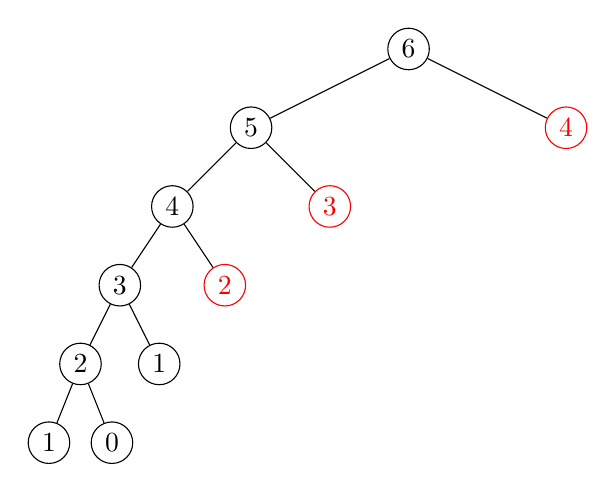
\begin{tikzpicture}
    \node {6}
      child { node {5}
        child { node {4} 
          child{ node {3} 
            child { node {2}
              child {node {1}}
              child {node {0}}
            }
            child { node {1}}
          }
          child{ node[color=red] {2} }
        }
        child { node[color=red] {3} }
      }
      child { node[color=red] {4}
      };
  \end{tikzpicture}
  \caption{Fibonacci recursion tree with $n = 6$}
  \label{fig:fib1}
\end{figure}

The red nodes in figure \ref{fig:fib1} still have to be visited by the algorithm, and they are expanded all 
way down into a node with label one or zero, even though if the answer was already computed in any other 
branch of the tree. This repetitive computation slows down the program drastically as n grows,
you can see that the number of nodes grows exponentially, since for every level we traverse down,
the number of nodes potentially double: the time complexity for this algorithm is $O(2^n)$, which is 
the number of nodes.

\begin{figure}[ht]
  \centering
  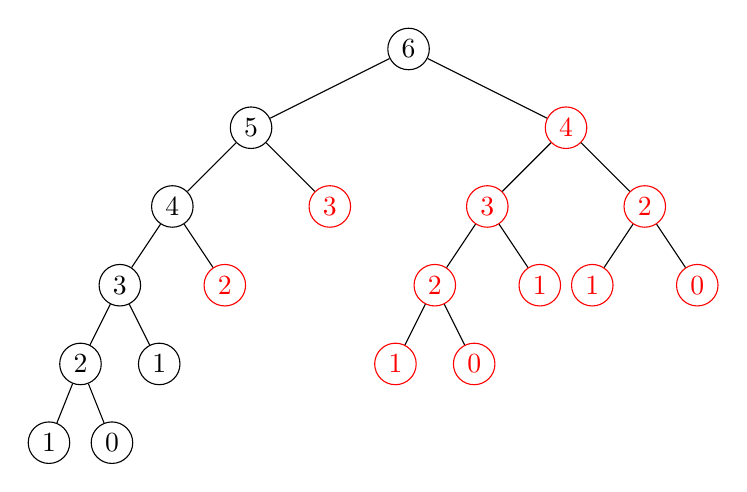
\begin{tikzpicture}
    \node {6}
      child { node {5}
        child { node {4} 
          child{ node {3} 
            child { node {2}
              child {node {1}}
              child {node {0}}
            }
            child { node {1}}
          }
          child{ node[color=red] {2}}
        }
        child { node[color=red] {3}}
      }
      child { node[color=red] {4}
        child{ node[color=red] {3} 
            child { node[color=red] {2}
              child {node[color=red] {1}}
              child {node[color=red] {0}}
            }
            child { node[color=red] {1}}
          }
        child{ node[color=red] {2} 
            child {node[color=red] {1}}
            child {node[color=red] {0}}
        }
      };
  \end{tikzpicture}
  \caption{Expanded fibonacci recursion tree}
  \label{fig:fib2}
\end{figure}

in figure \ref{fig:fib2} we expanded one of the red nodes labeled with 4: it gets computed twice, completely.
expanding all the tree would show us that node 3 gets computed three times, node 2 gets computed five times.
if we chose n = 7, for example, node 2 would be computed eight times. This unnecessary repeated
computations are  what makes this algorithm so slow.

Now, what if instead of repeating all this computations, the answers are stored somewhere? Each
time the algorithm would start , it wouldinstead look up in some kind of record or table, 
and if it finds a value, it just simply returns the value found immediatly.


\begin{minted}{python}
# initialize the look up table with 
# non-recursively defined fibonacci numbers.
look_up_table = {
 0: 1,
 1: 1  
}

def dp_fibonacci(n):
  if (look_up_table.at(n)):
    return look_up_table.at(n)
  else :
    look_up_table[n] = dp_fibonacci(n - 1) + dp_fibonacci(n + 2)
    return look_up_table[n]
\end{minted}


applying this change to the algorithm, yields a linear run time $O(n)$. This is because instead of expanding the
nodes marked red, dp\_fibonacci just retrieves the value from a dictionary, which is $O(1)$. This
is a tremendous gain in performance.



\section{Elements of Dynamic Programming}

Having seen how beneficial Dynamic Programming can be, it would be logical to
try to adapt algorithms to use a Dynamic Programming similar approach, but this is not always possible.
A problem must have specific properties in order to be solved in a Dynamic Programming fashion. We have
mentioned this traits: Optimal Substructures and Overlapping Substructures.

\subsection{Optimal Substructures}

As we have seen in the Fibonacci example, solutions to problems are 
related to solution to its sub-problems. The Tree representation for Fibonacci 
makes this concept very clear: The solution to a node placed in a higher 
level depends on the solution to its sub-problems: the nodes situated under it.

In optimization problems, an optimal solution to a problem involves optimally
solving its subproblems. A useful to illustrate this is the rod-cutting problem:

\indent \emph{Abridged Problem Statement}: given a rod of length n, and a table of prices $p_i$ for $i = 1, 2, ..., n$,
determine the maximum revenue $r_n$ obtained by cutting the rod and selling the pieces \cite{cormen2009introduction}

Suppose we have the following price table:
\begin{table}[ht]
\centering
\begin{tabular}{l|ll}
  \textbf{length i}&\textbf{price $p_i$}\\\hline
  1 & 2\\
  2 & 6\\
  3 & 7\\
  4 & 8\\
  5 & 9
\end{tabular}
\caption{Price Table for the rod-cutting problem}
\label{fig:priceforrods}
\end{table}

Having a rod of length $l = 1$ is quite trivial, the optimal solution is to leave the rod as it is, as we 
assume it cannot be cut furthermore. a road of length $l = 2$ is already at optimal length,
as its selling price 6 is higher than selling two rods of length $l = 1$ for a total of 4.
We see for example of length $l = 3$ that the optimal solution is cutting once, leaving
a rod of length $l = 2$ and a rod of length $l = 1$, for a total of $r = 8$. We can see that the optimal
solution to a road of length n involves considering  all posible ways of cutting the rod which
may range from 1 up to $n - 1$, as well as considering not cutting the rod, as was the case in length
$l = 2$. cutting a rod at length k creates two sub problems, ranging from 
$1 - k$ and $k+1 - n$. Both of these problems must be optimally solved in order to obtain max revenue.

For example, having a rod of length $l = 5$, we cut the rod at $k = 2$, leaving us with rods of length
$l = 2$ and length $l = 3$, if we were to cut the first road again, we will loose revenue, this road is already
optimally cut. But we can the rod of length $l = 3$ into pieces of lengths $l = 2$ and $l = 1$, for a total revenue of
14. If we were to sell the rod uncut, $l = 5$,  we would receive only a revenue of 9.


\subsection{Overlapping Subproblems}

There is another key property which a problem must posses, for Dynamic Programming to
be applicable. Often times the Search Space of the problem at hand is relatively small,
but naive solutions revisit the same problems over and over, as we have seen in the red
nodes in the Fibonacci example, in Figure \ref{fig:fib2}

When an algorithm revisits the same problem repeatedly, Cormen et. al. have coined the term
that the problem at hand has \emph{Overlapping Subproblems}.

Dynamic Programming solutions take advantage of this property and store the solution
of known problems in a data structure, so when this problem is encountered again, 
the algorithm takes constant time solving it, just by performing a look up at the Data
Structure. In our Fibonacci case, this would be our dicionary called \texttt{look\_up\_table}
\section{Matrix-Chain Multiplication}

The Matrix-Chain Multiplication problem is another example in which we can 
apply Dynamic Programming, yielding important performance gains.

Suppose we have a product (also called chain) of Matrices, numbered from 1 to n. Their product is
calculated as follows:

$$A_1A_2A_3...A_n$$

The number of scalar multiplications that have to be performed when multiplying matrices $A_1$
and $A_2$ with dimensions $m_1xn_1$ and $m_2n_2$ is equal to $m_1n_1n_2$ (remember that
for a two matrices, rows and columns must match in their number, else the matrices are not 
compatible and the multiplication cannot be performed). 

Now, how does this problem even relate to Dynamic Programming? remember that Matrix 
multiplication is \emph{associative} which means that parenthesization does not alter
the end result, in other words: $((A_1A_2)A_3) = (A_1((A_2A_3))$.

The product obtained by this multiplication will not vary with the way we parenthesize,
but the ammount of multiplications required may very well vary. Suppose we have
matrices of dimensions 3x50, 50x2 and 2x40, the first parenthesization yields 
3x50x2 + 3x2x40 = 540 multiplications, while the second variant yields
50x2x40 + 3x50x40 = 10000 multiplication, an almost scandalous difference.

\begin{quote}How we parenthesize a chain of matrices can have a dramatic impact of evaluating
the product \cite{cormen2009introduction}\end{quote}

the abridged problem statement can be written down as follows: given a n chain of matrices,
find a parenthesization with the least ammount of multiplications. These matrices are compatible
for multiplication, and for $i = 1, 2, ..., n$ the matrix $A_i$ has dimension $p_{i-1} * p_i$

Brute forcing this problem:


catalan numbers formula


Complexity


complexity new algo

new algo description

new algo graphics
\section{Solving Dynamic Programming Problems}

A general way to solve Dynamic Programming problems, as seen in \cite{cormen2009introduction}:

\begin{enumerate}
  \item Characterize the structure of an optimal solution.
  \item Recursively define the value of an optimal solution.
  \item Compute the value of an optimal solution, typically in a bottom-up fashion.
  \item Construct an optimal solution from computed information.
\end{enumerate}

\subsection{State and Recurrences}
\section{Dynamic Programming in Programming Contests}

\subsection{Classical Problem Types}

\subsubsection{Knapsack Problem}

\subsubsection{Coin Exchange}
\section{Top-down vs Bottom-up}

We have seen that two common ways to apply Dynamic Programming are using the top-down approach with memoization
and the bottom-up method. 


\bibliographystyle{acm}
\bibliography{references.bib}

\end{document}